% This document is compiled using pdfLaTeX
% You can switch XeLaTeX/pdfLaTeX/LaTeX/LuaLaTeX in Settings
\documentclass{article}
\usepackage{graphicx}
\usepackage{float}
\usepackage{verbatim}
% \usepackage{epstopdf}
% \epstopdfsetup{outdir=./}
\newcommand{\Class}{Operating system 2022}
\newcommand{\ClassInstructor}{Xu Wei}

% Homework Specific Information. Change it to your own
\newcommand{\Title}{Project 3}
\newcommand{\DueDate}{Dec 18, 2022}

% In case you need to adjust margins:
\topmargin=-0.45in      %
\evensidemargin=0in     %
\oddsidemargin=0in      %
\textwidth=6.5in        %
\textheight=9.0in       %
\headsep=0.25in         %

% Setup the header and footer
%\pagestyle{fancy}                                                       %
%\lhead{\StudentName}                                                 %
%\chead{\Title}  %
%\rhead{\firstxmark}                                                     %
%%\lfoot{\lastxmark}                                                      %
%%\cfoot{}                                                                %
%%\rfoot{Page\ \thepage\ of\ \protect\pageref{LastPage}}                          %
%\renewcommand\headrulewidth{0.4pt}                                      %
%\renewcommand\footrulewidth{0.4pt}                                      %


% Make title
\title{\textmd{\textbf{\date{}} \Class: \Title}\\{\large Instructed by \textit{\ClassInstructor}}\\\normalsize\vspace{0.1in}\small{Due\ on\ \DueDate}}

\author{\textbf{\StudentName}\ \ \StudentClass\ \ \StudentNumber}
%%%%%%%%%%%%%%%%%%%%%%%%%%%%%%%%%%%%%%%%%%%%%%%%%%%%%%%%%%%%%

\begin{document}
    % \begin{spacing}{1.1}
    % \maketitle \thispagestyle{empty}
    % \cite{}
% %%%%%%%%%%%%%%%%%%%%%%%%%%%%%%%%%%%%%%%%%%%%%%%%%%%%%%%%%%%%%
% % Begin edit from here
% \section*{Evaluation}
% \subsection*{C++}
%
%
% \subsection*{Go}
%
%
%
%
% \end{spacing}
    \section{Part 1 - Blockchain Design}\label{sec:part-1---design}
    \subsection{Client Transaction}

    Initially, we define a transaction structure which includes a timestamp and a string. To test the function of our blockchain, we randomly generates 100 strings as transactions, each node has 20 strings. Considering the real Bitcoin scenarios, the transactions in the network are generated faster than the blocks that the miners could find. Therefore, we set the frequency of creating a transaction as every five seconds after it's last broadcast transaction. Also, because we have more transactions, we need a queue to store the unsolved transactions. Here, we use a double linked list to realize a transaction pool.

    There are two primary functions for the transaction pool, insert and delete. Because, we want the node to process the transactions by created order, therefore every time we insert a new transaction, we arrange its position by its timestamp. Here we make an \textbf{assumption} that the clock of every machine is world clock. Therefore, we directly take the time of the node created as its order. If there are two transactions that accidentally take the same timestamp, which actually is a very small probability event, the transaction pool will order them by their sequence of coming. What's more, when deleting a transaction, we find from the list's head and if the transaction node's timestamp and transaction content are both the same then delete the corresponding node.

    To be specific, our transaction pool is a double linked list with transaction node ordered in their timestamp. 
    \subsection{Blockchain Structure}

    We first design the structure of the block to be broadcast, which contains the timestamp, hash of previous block, hash itself, nonce and the transaction data. This is the structure of the block to be broadcast to other nodes, while we also design another block structure used for building the offline blockchain. This blockNew contains the above block structure, along with a label representing its position in a chain and a pointer to its previous block.

    Then we design the structure of the blockchain, since each block in the chain has a pointer to its previous block, we only store the start block and an array of the tail blocks due to fork. Also we store the number of tails in the current chain.

    There are several related functions about how to build and maintain the offline blockchain. First we talk about how to compute the hash function value. We combine the hash of previous block, the transaction data and the timestamp to a long byte array and then use the SHA256 hash function to compute the hash of this block. Second, to start a chain, we construct the genesis block and add it as both start and tail block for the initial chain. Third, when receiving a new block, we use AddBlock function to add it to the offline chain. In this function, we first find for each tail whether the prevHash of the new block matches with their hash. If yes, we set the pointer of previous block to this tail lock and update the block in the tail array. If not, then traverse all chains to find its previous block and add this block as a new tail. Here we make an \textbf{assumption} that each block received can find an existing block which matches the PrevHash with it. Finally, there are two functions about the longest chain. One is about finding the tail block with the largest label, which means the chain ended with this block is the longest. This function returns the hash of this block, and the other returns the length of this chain. Apart from these, we also design check function, which checks the hash along the chain.

    \subsection{Proof of Work}
    Our target of PoW is to compute the nonce that makes the hash of the block be smaller than the targets. Therefore, we set an adjustable target that could control the speed of pow finding correct nonce. The target is the number of zero bits in the front of a binary number. Every time before we start to compute proof of work, we need to have a new block. Therefore, we implement a \verb|NewBlock()| that takes a hash value as an input. Here, we will give the result of longest chain function in the blockchain structure as the input to \verb|NewBlock()| because we want it always generates block on the longest chain. What's more, the new block's transaction is the head in the transaction pool. It is because we want to first add the eldest transaction into the chain. 

    After generating the new block and getting the target, we could start compute the nonce. Initially, we join the block's timestamp, previous hash and data's timestamp, transaction to an array of byte. And compute the nonce from 0. We join the array with nonce and compute its hash use SHA256. If the hash number is smaller than the target, we set the block's nonce and hash as the computed value and announce that I have done the proof of work. Else, add nonce by one and enter the for loop again. Additionally, we use a \verb|breakPow| variable to monitor the for loop. If there is any block broadcast to this node, it need to update its chain and its transaction pool. As a result, its information for new block may be changed. Therefore, we will set \verb|breakPow| as true and let it end this proof of work and start a new one with new block. While, accounts to our strategy of broadcast, here we wouldn't set the \verb|breakPow| of broadcaster as true.
  
    \subsection{Broadcast and Listen}
     Every time a client creates a transaction, which here means reading a line from our prepared document, it broadcasts the transaction to all the five nodes. Every time a miner finds a nonce, it broadcasts the \verb|BlockBroad| to all the five nodes. Therefore, our strategies for broadcast transaction and block are the same. Our target of broadcast is to add the corresponding transaction and block to every nodes' transaction pool and block chain. Here, we include the generator of the transaction or the block to the list of broadcast to cut down the difficulty of maintain the static address list. Also we don't need to locally update the transaction pool or block chain after generation.

     The realization of broadcast includes two functions, \verb|call(addr)| and \verb|broadcast()|. Because we need to send a complex structure to other nodes, here we use json marshal and unmarshal to serialize our messages. In the \verb|call(addr)| function, after the serialization, we use a simple rpc call to the remote server with address \verb|addr| and get the reply. In the \verb|broadcast()| function, we loop all the address in the static list and go \verb|call(addr)|.

     According to the broadcast, we register two services in the listen realization, \verb|Listen()| and \verb|ListenB()|. The \verb|Listen()| service is for listening transactions. Therefore, it will first unmarshal the request and then insert it to the transaction pool. The reply is "ACKT". The \verb|ListenB()| service is for listening blocks. It will also unmarshal the request, and delete the corresponding data in its transaction pool, add the block into the chain. The reply is "ACKB". After receiving \verb|ListenB()|, it needs to set the \verb|breakPow| which mentioned before as true. Then it will be broken from the for loop of currently running PoW. We use the same listening process as project 2, which is the rpc package in go.  
     
    \section{Part 2 - Evaluation}\label{sec:part-rvevaluatioern}
    In this part, we mainly talk about some metrics we evaluated for the blockchain, including the total time to construct the chain with 100 blocks, the number of block for each node to mine and the length of the longest chain.
    \subsection{Total Time}
    For each node, we evaluate its time from starting the process to finishing the chain of 100 blocks as shown in the figure. We also compute the average time and maximum time for all the nodes, which can be evaluated as the total time for the blockchain to mine 100 blocks. 
    \begin{figure}[H]
        \centering
        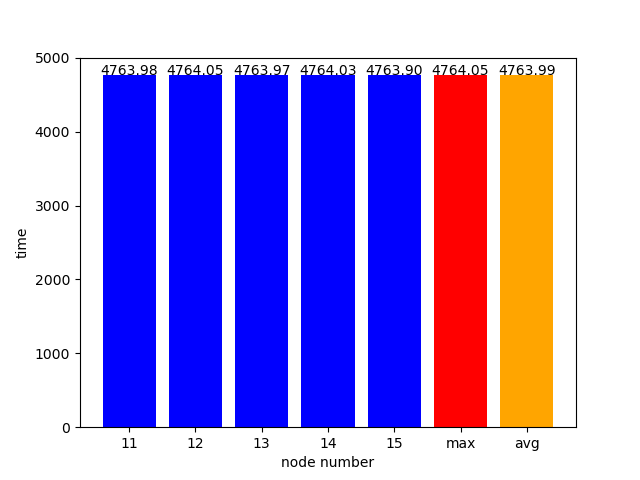
\includegraphics[width=10cm]{./eval/time.png}
        \caption{Total time for the process}
        \label{fig:my_label}
    \end{figure}
    From the figure we can see that the time for each block is slightly different, which results from the time of broadcasting blocks.
    \subsection{The Number of Block}
    We count the number of blocks mined by each node as shown below, where we totally request to mine 100 blocks. Also we compute the sum and variance of the data of block number, so that we can check how many blocks are mined and quantify the different mining ability of each block.
    \begin{figure}[H]
        \centering
        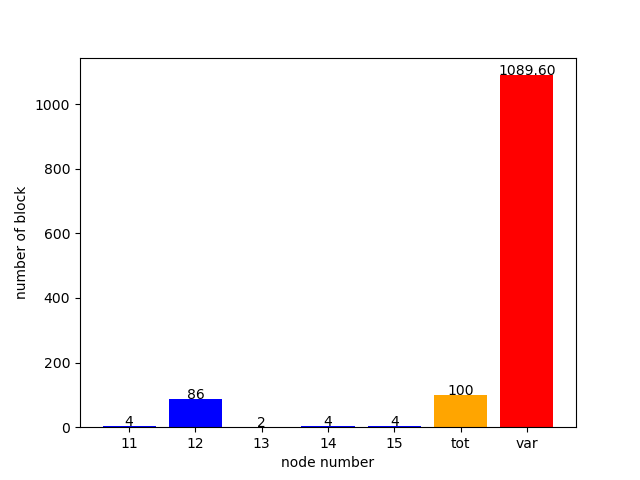
\includegraphics[width=10cm]{./eval/block.png}
        \caption{The number of block created by each node}
        \label{fig:my_label}
    \end{figure}
    Also from the figure above, we can see that the ability for each node to mine differs very much. And for some cases, we may find the sum is not 100, this is because there may exist fork and different node may use the same transaction to mine blocks.
    
    \subsection{The Length of the Longest Chain}
    In this part, we quantify the length of the longest chain in the blockchain in each node. Actually, we should have for certain that the length of the longest chain should be the same for each node and if there is fork then the length should be less than 100 because we totally mine 100 blocks.
    \begin{figure}[H]
        \centering
        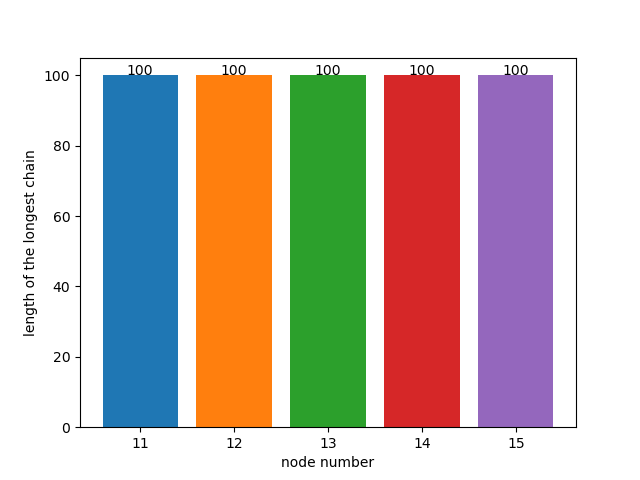
\includegraphics[width=10cm]{./eval/long.png}
        \caption{The length of the longest chain for each node}
        \label{fig:my_label}
    \end{figure}
    As we can see in this trial (not necessarily the same for the figure presented now), the process of mining a blockchain has no fork and just forms a single long chain of 100 blocks.
    \section{Part 3 - Omissions and Changes}\label{sec:part-2---omissions&changes}
    Initially, we make an assumption that the machines will not leave the network during our process. Therefore, we don't need to handle the error of rpc not connected. What's more, we also make an omission that we won't deal with the transaction that is on the orphan chain. Actually, in our evaluation process, fork happens with very small probability. Last, we make a change that every time we only process with one transaction. Every time, we just get one transaction out of the transaction pool and use it to do the PoW. We will do some improvement on this change in the following work.
    
    \section{Part 4 - Improvement proposals}
    \subsection{Merkle Tree}
    We designed another protocol of storing the transactions with Merkle tree. For a given block, we can only store the root of the Merkle tree instead of the whole information of transactions. And this can improve the performance of confirmation and validation of transactions when receiving new ones, because originally we need to check the transactions line by line to see whether there is modification, but with Merkle tree we can only check the root since the hash value is hard to hack. For this improvement, we can evaluate by the time spent on confirming the transactions and the space usage for each block.

    \subsection{Consensus policy: k-delay confirmations}
    We plan to design k-delay confirmation policy when faced with fork condition. Now we just store all possible forks locally and whenever receiving a new block, the miner will recheck the chain to find the longest one, change its choice of previous block and restart to compute the if necessary. With the k-delay confirmation policy, we will abort the fork with more than or equal to k delays. Then in this proposal we can improve the space performance and reduce the time spent on choosing and shifting to the longest chain. We can evaluate this improvement from the space and time spent on maintaining the local structure of blockchain.

    \subsection{Transanction confirmation and incentive mechanism}
    We plan to design a mechanism for transaction confirmation and incentive mechanism. After implementing the Merkle tree, we can confirm the transactions with the root of Merkle tree. And we also want to implement the incentive mechanism. As mining a block needs computational power and storage costs, we may need some incentive for mining to guarantee the participation and security of the blockchain. As we learned in the Internet, we can implement some related mechanism such as Fee and Waiting Tax mechanism or something else.

% \end{spacing}
\end{document}
